\documentclass{article}
\usepackage{geometry}
 \geometry{
 a4paper,
 total={170mm,257mm},
 left=20mm,
 top=20mm,
 }
\usepackage{graphicx}
\usepackage{titling} % Required for the custom subtitle hook
\usepackage{amsmath}
\usepackage{amssymb}
\usepackage{booktabs, bm}
\usepackage{tikz}
\usepackage{multirow}
\usepackage{multicol}
\usepackage{subcaption}
\usepackage{float}
\usepackage[round]{natbib}
\usepackage{pgfplots}
\pgfplotsset{compat=1.18}
\usetikzlibrary{positioning, arrows.meta, bending, calc}

\usepackage[capitalize,noabbrev]{cleveref}
\crefname{assumption}{Assumption}{Assumptions}
\usepackage{amsthm}
\usepackage{thmtools}
\usepackage{thm-restate}
\usepackage{tabularx}

% some definitions duplicated 
\declaretheorem[name=Theorem, numberwithin=section]{theorem}
\declaretheorem[name=Proposition, numberlike=theorem]{proposition}
\declaretheorem[name=Proposition, numberlike=theorem]{prop}
\declaretheorem[name=Lemma, numberlike=theorem]{lemma}
\declaretheorem[name=Lemma, numberlike=theorem]{lem}
\declaretheorem[name=Definition, numberlike=theorem]{definition}
\declaretheorem[name=Definition, numberlike=theorem]{define}
\declaretheorem[name=Corollary, numberlike=theorem]{cor}
\declaretheorem[name=Remark, numberlike=theorem]{remark}
\declaretheorem[name=Fact, numberlike=theorem]{fact}
\declaretheorem[name=Example, numberlike=theorem]{example}
\declaretheorem[name=Assumption, numberlike=theorem]{assumption}
\declaretheorem[name=Informal Theorem]{informalthm}

\usepackage{xcolor} % Required for text color
\newcommand{\todo}[1]{{\color{red}\bfseries [TODO: #1]}}
\newcommand{\russ}[1]{{\color{purple} (Russ: {#1})}}
\newcommand{\joseph}[1]{{\color{purple} (Joseph: {#1})}}


% Define the \subtitle command using titling hooks
\newcommand{\subtitle}[1]{%
  \posttitle{%
    \par\end{center}
    \begin{center}\large#1\end{center}
    \vskip0.5em}%
}

\title{Online Convex Optimisation Part II - Online Mirror Descent, Regret Bounds and Applications}
\subtitle{CS6216 Group 8a Reading Material}
\date{\today}
\author{
  Teoh Tze Tzun (\texttt{A0257871R})\thanks{These authors contributed equally to this work.} \qquad Tan Kai Min, Russell (\texttt{A0233120A})\footnotemark[1] 
}

\begin{document}
\maketitle
% \section{Introduction}
% \textit{Online learning} refers to a technique in machine learning and data science where a learner sequentially takes in data points and uses them to update itself gradually to improve its performance. This is opposed to offline learning, where there is already a set of data points which is readily available for the learner or the model to learn all at once. There have been many general online learning algorithms, such as \textit{mini-batch stochastic gradients descent}, \textit{passive-aggressive algorithms} and \textit{follow-the-leader}. We won't be covering these in this note. 

% \todo{\begin{enumerate}
%     \item What is Convex optimisation
%     \item How CO and OL marry into each other
%     \item General OCO framework
%     \item why CO
%     \item what this note will contain
% \end{enumerate}}

\begin{abstract}
    In online convex optimisation, a decision maker must iterative minimise cumulative loss in a dynamic environment. At each time step $t=1\ldots T$, the learner selects a decision vector $x^{(t)}$ from a convex feasible set. Only after committing to this choice does the environment reveal a convex loss function $f^{(t)}$, causing the learner to incur a loss of $f^{(t)}(x^{(t)})$. The core objective of the learner is to minimise the regret, defined as the the difference between the learner's accumulated loss over time and the total loss of the best possible fixed decision chosen in hindsight. Standard online gradient descent relies on Euclidean projections, which can be highly suboptimal for decision sets with distinct geometric structures, such as the probability simplex. Online Mirror Descent (OMD) is a fundamental algorithm that generalises classical gradient descent to non-Euclidean spaces. We provide an overview of online mirror descent, exploring its variants, regret bounds, and applications. We begin by reviewing foundational concepts from Week 7 that establish the basis for our analysis. Next, we introduce essential analytical tools before concluding with practical use cases.
\end{abstract}

% \section{Brief Recap of Part I}
% \russ{contemplating if we should do this or just ask people to read Part I from Week 7 people}
\section{Recap on Follow-The-Regularised-Leader}
This section will consist of a brief recap of the Follow-the-Regularised-Leader (FoReL) back in Week 7. FoRel is a simple modification of the Follow-The-Leader (FTL) learning rule.  In FTL, in each iteration, we select the decision vector (or the next iterate) which minimises the loss on all past iterations:
\begin{define}[Follow-The-Leader]
    The Follow-The-Leader (FTL) learning rule is as such: we select the next iterate my minimising the loss on all past rounds. That is for a convex set $S$,
    \begin{equation}
        \forall t\; x_t = \arg \min_{x \in S} \left\{\sum_{i = 1}^{t-1} f_i(x)\right\}
    \end{equation}
\end{define}
In FoRel, we add a regularisation term $h$. The goal of the regularisation term is to stabilise the solution.
\begin{define}[Follow-The-Regularised-Leader]\label{defn:forel} The Follow-The-Regularised-Leader (FoREL) learning rule extends FTL by adding a regularisation term $h: S \to \mathbb R$.
    \begin{equation}
        \forall t\; x_t = \arg \min_{x \in S} \left\{\sum_{i = 1}^{t-1} f_i(x) + h(x)\right\}
    \end{equation}
\end{define}

\subsection{Mathematical Preliminaries}
We also recap some of the important definitions that will be important in helping us understand the tools used for the analysis of regret bounds.

\begin{define}[L-Lipschitz]
    A function $f$ is called $L$-Lipschitz over a set $S$ with respect to a norm $||\cdot||$ if for all $x, x' \in S$, we have that \begin{equation*}
        |f(x) - f(x')| \leq L ||x - x'||
    \end{equation*}
\end{define}

\begin{define}[$\sigma$-strongly convex]\label{defn:sigma_strong_convexity}
    A function $f$ that is $\sigma$-strongly convex over a set $S$ with respect to norm $||\cdot ||$ if for any $x' \in S$, we have that \begin{equation*}
        \forall z \in \partial f(x'),\;\forall x \in S, \; f(x) \geq f(x') + \langle z, x - x' \rangle + \frac{\sigma}{2} || x - x' ||^2
    \end{equation*}
    where $\partial f(x')$ is the set of sub-gradients of $f$ at $x'$. Furthermore, if $x^*$ minimises $f$ over $S$, then for all $x' \in S$
    \begin{equation*}
        f(x') - f(x^*) \ge \frac{\sigma}{2}||x' - x^*||^2
    \end{equation*}
\end{define}

We also define something that might be unfamiliar to the reader which is called the \textit{dual norm}, denoted by $||\cdot||_*$
\begin{define}
    Let $||\cdot||$ be a norm. The dual norm of $||\cdot||$ is a function $||\cdot||_*$ defined as
    \begin{equation}
        ||y||_* := \sup\{\langle x, y \rangle: ||x|| \leq 1\}
    \end{equation}
\end{define}
The dual norm of the $\ell_2$-norm is again the $\ell_2$-norm (the $\ell_2$-norm is therefore \textit{self-dual}). In general, the dual for the $\ell_p$-norm is the $\ell_q$-norm, where $\frac{1}{p} + \frac{1}{q} = 1$. We also give a lemma for a convex function which is $L$-Lipschitz and how it relates to the dual norm.
\begin{lemma} Let $f: S \to \mathbb R$ be a convex function. $f$ is $L$-Lipschitz over $S$ with respect to a norm $||\cdot||$ if and only if for all $x'\in S$ and $z \in \partial f(x')$, we have $||z||_* \leq L$.
\end{lemma}
\subsection{Regret Bound Results for FoReL}
We give a proof sketch on deriving the regret bound for FoReL. From Week 7's notes, the regret for FoReL can be written as the following when evaluated against a fixed value $x$ as such:
\begin{equation}\label{eqn:regret_forel}
    \text{Regret}_T(x) := \sum_{t=1}^T f_t(x_t) - \sum_{t=1}^T f_t(x)
\end{equation}
To prove the bound for the above expression, recall also that we have the following lemma:
\begin{lemma}\label{lemma:iterates_forel}
    Let $x_1, x_2, \ldots$ be the iterates due to FoReL using the $\sigma$-strongly convex regulariser $h$. Then for all $x \in S$, we have that \begin{equation}\label{eqn:lemma_forel}
        \sum_{t=1}^T (f_t(x_t) - f_t(x)) \leq h(x) - h(x_1) + \sum_{t=1}^T (f_t(x_t) - f_t(x_{t+1}))
    \end{equation}
\end{lemma}
Furthermore, it is also shown that if for all $t$, if $f_t$ is $L_t$-Lipschitz with respect to $||\cdot||$, then we further have that 
\begin{equation}\label{eqn:lemma_forel_lipschitz}
    f_t(x_t) - f_t(x_{t+1}) \leq L_t ||x_t - x_{t+1}|| \leq \frac{L_t^2}{\sigma}
\end{equation} 
Again, interested readers may refer to Week 7's notes or \cite{shalev2025online} for the full derivation. Combining Equations~\ref{eqn:lemma_forel} and \ref{eqn:lemma_forel_lipschitz} we have that the regret bound for FoReL using the regulariser $h$ is as follows:
\begin{equation}\label{eqn:forel_regre_with_min}
    \text{Regret}_T(x) \leq h(x) - h(x_1) + \frac{TL^2}{\sigma} \leq h(x) - \min_{v \in S} h(v) + \frac{TL^2}{\sigma}
\end{equation} where $L$ is such that $\frac{1}{T}\sum_{t=1}^T L_t^2 \leq L^2$.

\subsection{The Problem with FoReL}
The main issue (or a disadvantage) is that for FoReL, we need solve an optimisation problem \textit{at every iteration}, which is computationally inefficient and might be extremely complex. This leads us to a very natural question: \textit{Can we achieve a similar regret bound with a simpler update rule?} It turns out that we indeed can achieve a much simpler update rule without worsening the regret bound by using the Online Mirror Descent (OMD) family of algorithms.
\section{An Introduction to Online Mirror Descent}
In this section, we aim to give an introduction to the Online Mirror Descent (OMD) framework and give a few variants of the online mirror descent algorithm alongside their regret bounds. However, before diving deep into the framework, it might be best to give an overview on what basic mirror descent is.

\subsection{Classical Mirror Descent}
We might have been familiar with iterative algorithms such as gradient descent, and from this class, the multiplicative weights update (MWU) algorithm to solve different classes of learning and optimisation problems. A generalisation of gradient descent and the MWU algorithm is the \textit{mirror descent algorithm}. Let us give an intuition on what mirror descent is by first studying the standard gradient descent algorithm. Given that the iterates of the standard gradient descent algorithm to be $x_1, x_2 \ldots, x_n, \ldots$, with learning rate $\eta$ to find the local minima of the objective function $f$. The next iterate step is as such:
\begin{equation}
    x_{t+1} = x_t - \eta \nabla f(x_t)
\end{equation}
There is an underlying assumption for this next iterate step: the iterates $x_t$ and the gradient value $\nabla f(x_t)$ lie in the same space (in fact, this is only uniquely true if both the iterate-space and the gradient-value space are Hilbert spaces endowed with an Euclidean $\ell_2$ inner product norm). Therefore, if you are optimising over the space where the $\ell_2$-norm geometry is unnatural (for example, $\Delta_n$, a $n$-dimensional simplex), then standard gradient descent would be very slow as the dimensions increase.

To resolve this mismatch in the geometries of the spaces of iterates and gradients, Nemirovski and Yudin \citep{nemirovskij1983problem} then proposed the following framework whereby we treat the iterates and its corresponding gradients as residing in \textit{two distinct spaces}. Specifically, $x_t$ belongs to what we call the \textit{primal space} $\mathcal{X}$, and its corresponding gradient $\nabla f(x_t)$ will belong to the \textit{dual space} $\theta$ (which is natural since the gradient is defined as a linear functional in $\mathbb{R}^n$). The general idea of this framework is therefore we first ``map" the iterate $x_t$ via some mapping into the dual space, do a gradient step and then ``map" it back to the primal space to get $x_{t+1}$. The question that follows is how do we go about this ``mapping".

\subsubsection{Mapping from Primal Space to Dual Space}
To define this map, we must first fix a norm $||\cdot||$ and then choose some differentiable, convex function $h: \mathbb{R}^n \to \mathbb{R}$ that is $\sigma$-strongly convex.
Using $h$, we can define a \textit{distance} which quantifies how much the function differs from its linear approximation. We call it the \textit{Bregman Divergence}. With that, $h$ can be thought of as some ``distance-generating function".
\begin{define}[Bregman Divergence]\label{defn:bregmann_div}
    The Bregman divergence with respect to a strictly convex function $h$ (denoted by $D_h$), of two points, $x$ and $x'$ is defined as follows:
    \begin{equation}
        D_h(x || x') := h(x) - h(x') - \langle\nabla h(x'),  x - x' \rangle
    \end{equation}
\end{define} 
Figure~\ref{fig:bregman-divergence} gives an illustration on what the Bregman divergence entails. We will see the Bregman divergence in the later sections in the regret analysis of some online mirror descent algorithms, but for now, we will see how we derive the mapping from the primal space to the dual space.
% fig-bregman-divergence.tex
% Requires in the main preamble:
%   \usepackage{amsmath,amssymb}
%   \usepackage{tikz}
%   \usetikzlibrary{arrows.meta,bending,calc}
\begin{figure}[h!]
  \centering
  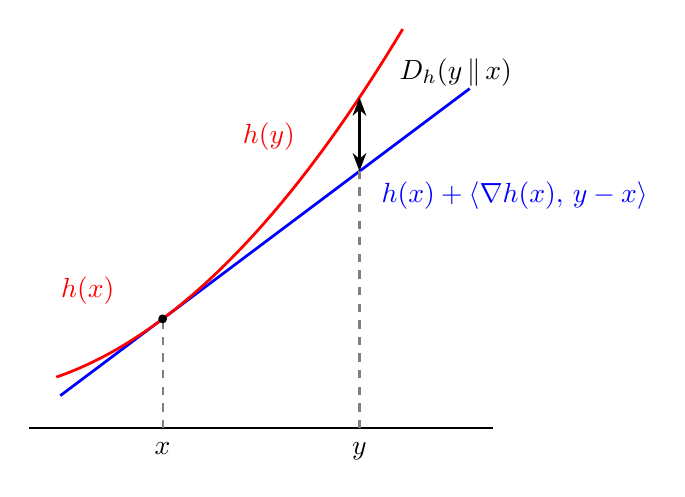
\begin{tikzpicture}[>=Stealth, line width=0.8pt,
                      declare function={h(\t)=0.15*\t*\t+0.3*\t+0.6;}]

    % ---------- axis ----------
    \draw[-] (-0.2,0) -- (5.7,0);

    % ---------- key abscissae ----------
    \def\xx{1.5}   % x
    \def\yy{4.0}   % y
    % h(x)=1.3875, h'(x)=0.75  ->  tangent L(t)=h(x)+h'(x)(t-x)
    \def\hx{1.3875}
    \def\slope{0.75}

    % ---------- tangent / linear approximation (blue) ----------
    \draw[blue,line width=1pt]
      (0.2,{\hx+\slope*(0.2-\xx)}) -- (5.4,{\hx+\slope*(5.4-\xx)});

    % ---------- convex function h (red) ----------
    \draw[red,line width=1pt,smooth,samples=100,domain=0.15:4.55]
      plot (\x,{h(\x)});

    % ---------- dashed drop lines ----------
    \draw[dashed,gray] (\xx,0) -- (\xx,{h(\xx)});
    \draw[dashed,gray] (\yy,0) -- (\yy,{h(\yy)});

    % ---------- Bregman gap at y ----------
    \draw[<->] (\yy,{\hx+\slope*(\yy-\xx)}) -- (\yy,{h(\yy)});
    \node[anchor=west] at (\yy+0.38,4.52) {$D_h(y\,\|\,x)$};

    % ---------- point at (x,h(x)) ----------
    \fill (\xx,{h(\xx)}) circle (1.6pt);

    % ---------- curve / line labels ----------
    \node[red]  at (2.85,3.7) {$h(y)$};
    \node[red]  at (0.55,1.75) {$h(x)$};
    \node[blue,anchor=west] at (4.15,2.95)
      {$h(x)+\langle \nabla h(x),\, y-x\rangle$};

    % ---------- axis ticks ----------
    \node[below] at (\xx,-0.05) {$x$};
    \node[below] at (\yy,-0.05) {$y$};

  \end{tikzpicture}
  \caption{The Bregman divergence $D_h(y\,\|\,x)$ is the gap at $y$ between the
    convex function $h$ and its linear (first-order) approximation
    $h(x)+\langle \nabla h(x),\, y-x\rangle$ taken at $x$.}
  \label{fig:bregman-divergence}
\end{figure}
\paragraph{The Mirror Map}
Nemirovski and Yudin defined the map from $\mathcal X$ to $\theta$ to be known as the \textbf{\textit{mirror map}}. Having fixed $||\cdot||$ and $h$, the mirror map is: \begin{equation}
    \nabla h: \mathbb R^n \to \mathbb R^n
\end{equation} Since $h$ is differentiable and strongly convex, we can easily define the \textit{inverse map} as well. We will now show why $\nabla h$ is the mirror map. Suppose we have a single proximal gradient step:
\begin{equation}\label{eq:proximal_gradient_update}
    x_{t+1} = \arg \min_{x} \left\{\eta \langle \nabla f(x_t), x\rangle + R(x)\right\}
\end{equation} where $R$ is some regularisation function. Suppose $R(x) = \frac{1}{2}||x - x_t||^2$, then solving the minimisation problem in Equation~\ref{eq:proximal_gradient_update} will yield the standard gradient descent update step. For our case, however, we let $R(x) = D_h(x || x_t)$. Therefore we have:
\begin{align}
    x_{t+1} &= \arg \min_{x} \left\{\eta \langle \nabla f(x_t), x\rangle + D_h(x ||x_t)\right\}
\end{align}
Solving the minimisation problem, we set the gradient of $x$ to be 0 (note, the minimiser $x^*$ will be the value of the next iterate, assuming an unconstrained problem):
\begin{align*}
    &\nabla(\eta \langle \nabla f(x_t), x\rangle + D_h(x^* ||x_t)) = 0\\
    \implies&\eta \nabla f(x_t) + \nabla D_h(x^*||x_t) = 0\\
    \implies& \eta \nabla f(x_t) + \nabla (h(x^*) - h(x_t) - \langle \nabla h(x_t), x^* - x_t \rangle) = 0\\
    \implies&\eta \nabla f(x_t) + \nabla h(x^*) - \nabla h(x_t) = 0
\end{align*}Note that $\nabla h(x_t)$ is constant w.r.t $x^*$. Rearranging the final step yields \begin{equation}
    \nabla h(x^*) = \nabla h(x_t) - \eta \nabla f(x_t) \implies \boxed{\nabla h(x_{t+1}) \gets \nabla h(x_t) - \eta \nabla f(x_t)}
\end{equation} Notice how the typical gradient descent update step has changed from iterating in terms of $x$ to $\nabla h(x)$. Therefore the mirror map is defined as $\nabla h$ and that $\theta_t = \nabla h (x_t)$. We can now move to formally state the mirror descent algorithm.

\subsubsection{Mirror Descent Algorithm}
Now, let us formally state the algorithm. Suppose we want to minimise a convex function $f$ over some convex set $S \subseteq \mathcal X$. We fix a norm $||\cdot ||$ on $\mathcal X$ and choose a function $h : \mathcal X \to \mathbb R$, which yields a mirror map $\nabla h : \mathcal X  \to \theta$. For each iteration, we do the following:
\begin{enumerate}
    \item Suppose we have the current iterate $x_t$, map it to its dual space to obtain $\theta_t = \nabla h(x_t)$
    \item Take a gradient step: $\theta_{t+1} \gets \theta_t - \eta\cdot \nabla f(x_t)$
    \item Using the inverse map $(\nabla h)^{-1}$, get back a point in the primal space: $x'_{t+1} \gets (\nabla h)^{-1}(\theta_{t+1})$
    \item Project $x'_{t+1}$ back to the feasible region $S$. If $x'_{t+1} \in S$, then $x_{t+1} = x'_{t+1}$, otherwise, we utilise the Bregman divergence and set $x_{t+1} = \min_{x \in S} D_h(x||x'_{t+1} )$.
\end{enumerate}
Figure~\ref{fig:mirror_descent} gives an illustration of the steps described above.
\begin{figure}[h!]
\centering
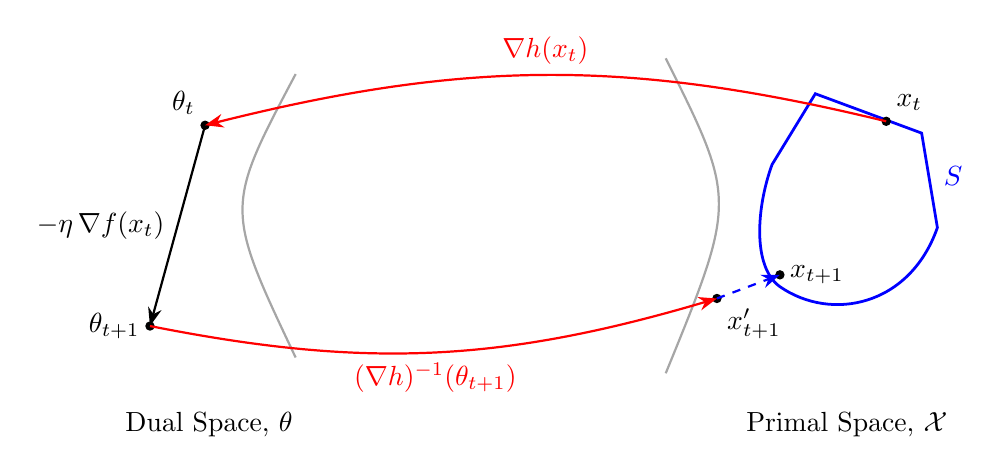
\begin{tikzpicture}[>={Stealth[bend]}, line width=0.8pt]
 
% ---------- space boundary curves ----------
% dual-space boundary (open arc, bulging right)
\draw[gray!70] (2.4,3.3) .. controls (1.5,1.6) .. (2.4,-0.3);
% primal-space boundary (open arc, bulging left)
\draw[gray!70] (7.1,3.5) .. controls (8.0,1.7) .. (7.1,-0.5);
 
% ---------- convex feasible set X (primal) ----------
\coordinate (xt)   at (9.9,2.7);   % x_t
\coordinate (xtp)  at (8.55,0.75); % x_{t+1}   (on boundary of X)
\coordinate (xppt) at (7.75,0.45); % x'_{t+1}  (outside X)
 
\draw[blue,line width=1pt]
  (9.0,3.05) -- (10.35,2.55) -- (10.55,1.35)
  .. controls (10.2,0.35) and (9.2,0.15) .. (8.55,0.6)
  .. controls (8.2,0.85) and (8.25,1.6) .. (8.45,2.15)
  -- cycle;
\node[blue] at (10.75,2.0) {$S$};
 
% ---------- dual points ----------
\coordinate (tt)  at (1.25,2.65);  % theta_t
\coordinate (ttp) at (0.55,0.10);  % theta_{t+1}
 
% ---------- markers ----------
\foreach \p in {tt,ttp,xt,xtp,xppt}{\fill (\p) circle (1.7pt);}
 
% ---------- point labels ----------
\node[above left]  at (tt)   {$\theta_t$};
\node[left]        at (ttp)  {$\theta_{t+1}$};
\node[above right] at (xt)   {$x_t$};
\node[right]       at (xtp)  {$x_{t+1}$};
\node[below right] at (xppt) {$x'_{t+1}$};
 
% ---------- dual update (gradient step) ----------
\draw[->] (tt) -- node[left=1pt]{$-\eta\,\nabla f(x_t)$} (ttp);
 
% ---------- mirror maps (red, bowed outward) ----------
\draw[red,->] (xt)  to[bend right=14] node[above]{$\nabla h(x_t)$} (tt);
\draw[red,->] (ttp) to[bend right=14] node[below]{$(\nabla h)^{-1}(\theta_{t+1})$} (xppt);
 
% ---------- Bregman projection onto X ----------
\draw[blue,dashed,->] (xppt) -- (xtp);
 
% ---------- region captions ----------
\node at (1.3,-1.15) {Dual Space, $\theta$};
\node at (9.4,-1.15) {Primal Space, $\mathcal X$};
 
\end{tikzpicture}
\caption{Illustration of Mirror Descent}
\label{fig:mirror_descent}
\end{figure}

\subsection{Online Mirror Descent}
We now focus on online mirror descent. Fundamentally speaking, both versions of mirror descent are similar in terms of the update rule but different in the following ways:\begin{enumerate}
    \item \textbf{Objective Function} The objective function for online mirror descent changes at every step. At step $t$, the algorithm must commit to a prediction $x_t$ before the ``environment" reveals the specific loss function $f_t$ for that iteration.
    \item \textbf{Gradient} In online mirror descent, we use the \textit{sub-gradient} of the newly revealed function $f_t$ for that iteration. We denote the sub-gradient as $z_t \in \partial f_t(x_t)$. This implies that the update rule is now \begin{equation}
        \theta_{t+1}=  \theta_t - \eta \cdot z_t\qquad z_t \in \partial f_t(x_t)
    \end{equation}
\end{enumerate}
A sub-gradient of a function is a more generalised form of a gradient. More specifically, we define sub-gradients as follows:\begin{define}[Sub-gradients]\label{defn:subgradient}
    A value $z$ is a sub-gradient of $f$ at $x$ if for all $x' \in S$\begin{equation}
        f(x') \geq f(x) + \langle x' - x, z\rangle
    \end{equation}
    The set of sub-gradients of $f$ at $x'$ is denoted by $\partial f(x')$. Furthermore, if $f$ is differentiable at $x'$, then $\partial f(x') = \{\nabla f(x')\}$ (i.e $\partial f(x^*)$ is a singleton and its only element is the gradient of $f$ at $x'$).
\end{define}


\subsection{Generic Regret Bound for Online Mirror Descent (OMD) Algorithms}
As you would have realised, the many different variants of online mirror descent algorithms are typically characterised by the geometries of the primal and dual space and, by relation, the mirror map $\nabla h$. That is to say, if $h$ changes (hence $\nabla h$ changes), then the update rule would look very different. 

Let us first reframe the mirror map $\nabla h$. Since $h$ is strictly convex, the inverse mapping exists, and therefore the next iterate can be written as \begin{equation}\label{eqn:x_t+1_g}
    x_{t+1} \gets (\nabla h)^{-1}(\theta_{t+1}) =: g(\theta_{t+1})
\end{equation} We will now rewrite $g$ into a form which will be useful to our analysis of different variants of the OMD algorithm. Starting off from the proximal gradient step:
\begin{align*}
    x_{t+1} &= \arg \min_{x} \left\{\eta \langle \nabla f_t(x_t), x\rangle + D_h(x || x_t)\right\}\\
    &=\arg\min_x \{ \eta \langle \nabla f_t(x_t), x \rangle + h(x) - h(x_t) - \langle \nabla h(x_t), x - x_t \rangle \}\\
    &=\arg\min_x \{ \eta \langle \nabla f_t(x_t), x \rangle + h(x) - \langle \nabla h(x_t), x \rangle \} &\because \,h(x_t), x_t \text{ are constants}\\
    &=\arg\min_x \{ h(x) - \langle \nabla h(x_t) - \eta \nabla f_t(x_t), x \rangle \} &\because \text{factor out }x\\
    &=\arg\min_x \{ h(x) - \langle \theta_{t+1}, x \rangle \}&\because\,\theta_{t+1} =\nabla h(x_t) - \eta \nabla f_t(x_t)\\
    &=\arg\max_{x} \{\langle \theta_{t+1}, x \rangle - h(x)\} \implies \boxed{g(\theta_{t+1}) = \arg\max_x \{\langle \theta_{t+1}, x \rangle - h(x)\}}
\end{align*}

\subsubsection{Relating FoReL with OMD}\label{sss:forel_OMD_relation}
We first establish some connection with FoReL and the OMD family of algorithms. Suppose we apply FoReL on a sequence of linear functions $f_t(x) = \langle x, z_t \rangle$ with some regulariser $h(x)$. For simplicity, we assume $h(x) = \infty$ if $x \notin S$. We start from the update rule of FoReL: \begin{align*}
    x_{t+1} = \arg\min_{x \in S} \left\{\sum_{i=1}^t f_i(x) + h(x) \right\} &= \arg\min_{x \in S} \left\{\sum_{i=1}^T \langle x, z_t \rangle  + h(x)\right\} \\&= \arg\max_{x \in S} \left\{\left\langle x, -\sum_{i=1}^T z_i \right\rangle - h(x)\right\}
\end{align*}
Comparing the expression with the equation $g$ we derived, we can easily make the substitution that $$\theta_{t+1} := \sum_{i=1}^t -z_i = \left(\sum_{i=1}^{t-1}-z_i\right) - z_t = \theta_{t} - z_t$$ This is exactly the update rule in the dual space as described in the OMD algorithm! It therefore also follows that $x_{t+1} = g(\theta_{t+1})$ as well, consistent with Equation~\ref{eqn:x_t+1_g}! By formalising this relationship, we can borrow some regret bounds results from FoReL and re-use them in analysing the regret bounds of OMD. Moreover, if $f_t$ is non-linear but still convex, we pick $z_t \in \partial f(x_t)$ and use a \textit{linearisation trick}: by the definition of a sub-gradient, we have that $f_t(x_t) - f_t(x) \leq \langle x_t - x, z_t \rangle = \langle x_t, z_t\rangle - \langle x, z_t \rangle$ which shows that the regret with respect to non-linear functions can still be upper bounded by that of linear functions.
\subsubsection{The Generic Regret Bound}
We now state the theorem of the generic regret bound for Online Mirror Descent (OMD) algorithms
\begin{theorem}[Generic Regret Bound Theorem for Online Mirror Descent Algorithms]\label{thm:generic_OMD_regret_bound}
    Let $h$ be a $\frac{1}{\eta}$-strongly convex function over $S$ with respect to a norm $||\cdot||$. Assume that we run Online Mirror Descent Algorithm on the sequence with \begin{equation}\label{eqn:g_argmax}
        g(\theta) = \arg\max_x \{\langle \theta, x \rangle - h(x)\}
    \end{equation}
    Then for all $x \in S$, we have that \begin{equation}
        \text{Regret}_T(x) := h(x) - \min_{v \in S} h(v) + \eta \sum_{t=1}^T ||z_t||_*^2
    \end{equation} where $||\cdot||_*$ is the dual norm and $z_t \in \partial f(x_t)$. Furthermore, if $f_t$ is $L_t$-Lipschitz with respect to $||\cdot||$, then we can further upper bound $||z_t||_* \leq L_t$.
\end{theorem}
\begin{proof}
    Firstly, since $z_t \in \partial f(x_t)$, then we have that for all $x \in S$:
    \begin{align*}
        &f_t(x) \geq f_t(x_t) +  \langle x - x_t, z_t \rangle &\because\,Definition~\ref{defn:subgradient}\\
        \implies &\sum_{t=1}^T (f_t(x) - f_t(x_t)) \geq \sum_{t=1}^T \langle x - x_t, z_t \rangle &\because \text{Summing over }1 \ldots T\\
        \implies &\sum_{t=1}^T (f_t(x_t) - f_t(x)) \leq \sum_{t=1}^T \langle x_t - x, z_t \rangle &\because \text{ Taking negatives}
    \end{align*}
    We know that the OMD algorithm is equivalent to running FoReL on the sequence of linear functions with regulariser $h$. We can start from Equation~\ref{eqn:lemma_forel_lipschitz}. Substituting $\sigma = \frac{1}{\eta}$ and then notice we can let $L_t = ||z_t||_*$ by observing the following: given that $f_t$ are linear functions, then the Lipschitz constant of the linear function with respect to the primal norm $||\cdot||$ is exactly equal to the dual norm of its sub-gradient $||z_t||_*$. We can see this relationship from the following sequence of inequalities: $f_t(x_t) - f(x_{t+1}) \leq \langle z_t, x_t - x_{t+1}\rangle\leq ||z_t||_* ||x_t - x_{t+1}||$ where the first inequality comes from the linearisation trick and the second inequality results from Holder's inequality. By Lemma~\ref{lemma:iterates_forel}, we have that:
    \begin{align*}
        \text{Regret}_T(x) &\leq h(x) - h(x_1) + \sum_{t=1}^T (f_t(x_t) - f_t(x_{t+1}))\\
        &\leq h(x) - h(x_1) + \sum_{t=1}^T (\frac{L_t^2}{\sigma})&\Cref{eqn:lemma_forel_lipschitz}\\
        &\leq h(x) - h(x_1) + \eta \sum_{t=1}^T ||z_t||_*^2 &\because \sigma = \frac{1}{\eta}\,,L_t = ||z_t||\\
        &\leq h(x) - \min_{v\in S}h(v) + \eta \sum_{t=1}^T ||z_t||_*^2&\because \min_{v \in S} h(v) \leq h(x_1)
    \end{align*}
\end{proof}

\subsection{Variants of OMD algorithms}
As mentioned before, the different variants of OMD algorithms can be characterised by the geometries of the primal and dual space and hence $g$. We will be introducing some of the variants in this subsection and their regret bounds.

\subsubsection{Normalised Exponentiated-Gradient (EG)}
Suppose our feasible set $S = \Delta_d = \{x \in \mathbb R^d_{\geq 0} \mid \sum_{i=1}^d x_i = 1\}$, which is a $d$-dimensional probability simplex, and that $h(x) = \frac{1}{\eta}\sum_{i=1}^d x_i \log x_i$, otherwise known as the \textit{entropic regulariser} which is itself $\frac{1}{\eta}$-strongly convex with respect to the $\ell_1$-norm. The following expression of $g$ is as such:
\begin{equation*}
    w_{t+1} = g(\theta_{t+1}) = \arg\max_{x \in \Delta_d} \left\{\sum_{i=1}^d \theta_{t+1,i}x_i - \frac{1}{\eta}\sum_{i=1}^d x_i \log x_i\right\}
\end{equation*}
To solve the above, we need to use the method of Lagrange multipliers (recall basic undergraduate calculus). We first set up the Lagrangian function $\mathcal L$ with respect to $x$ and the dual variable $\lambda$. The Langrangian can be written as:
\begin{equation}
    \mathcal L(x, \lambda) = \sum_{i=1}^d \theta_ix_i - \frac{1}{\eta}\sum_{i=1}^d x_i \log x_i + \lambda\left(1 - \sum_{i=1}^dx_i \right)
\end{equation}
Taking the derivative with respect to a component in $x_i$ yields:\begin{equation*}
    \frac{\partial \mathcal L}{\partial x_i} = \theta_{t+1, i}- \frac{1}{\eta}(\log x_i + 1) - \lambda = 0 \implies x_i = \exp(\eta \theta_{t+1, i})\exp(-1 - \eta \lambda)
    \end{equation*}
Since $\sum_{i=1}^d x_i = 1$, then $\sum_{j=1}^d \exp(\eta \theta_{t+1, j})\exp(-1 - \eta \lambda) = 1 \implies \exp(-1-\eta\lambda) = \frac{1}{\sum_{j=1}^d \exp(\eta \theta_{t+1, j})}$.
We therefore have the final expression $x_i = \frac{\exp(\eta \theta_{t+1, i})}{\sum_{j=1}^d \exp(\eta \theta_{t+1, j})}$. For those who have taken basic machine learning, we indeed see that $g$ is the softmax function. We can further give a recursive formula with respect to $x$-iterates as follows:
\begin{align*}
x_{t+1, i} &= \frac{\exp(\eta \theta_{t+1, i})}{\sum_{j=1}^d \exp(\eta \theta_{t+1, j})} = \frac{\exp(\eta \theta_{t+1, i})}{\sum_{j=1}^d \exp(\eta \theta_{t+1, j})} \cdot \frac{\sum_{k=1}^d \exp(\eta \theta_{t, k})}{\sum_{k=1}^d \exp(\eta \theta_{t, k})} \\
&= \frac{\exp(\eta \theta_{t, i}) \exp(-\eta z_{t, i})}{\sum_{j=1}^d \exp(\eta \theta_{t, j}) \exp(-\eta z_{t, j})} \cdot \frac{\sum_{k=1}^d \exp(\eta \theta_{t, k})}{\sum_{k=1}^d \exp(\eta \theta_{t, k})} \\
&= \frac{x_{t, i} \exp(-\eta z_{t, i})}{\sum_{j=1}^d x_{t, j} \exp(-\eta z_{t, j})}
\end{align*}
Therefore, the algorithm is as follows:
\begin{enumerate}
    \item Set $w_1 = (1/d, 1/d, \ldots, 1/d)$
    \item For all $i$: $x_{t+1, i} =\frac{x_{t, i} \exp(-\eta z_{t, i})}{\sum_{j=1}^d x_{t, j} \exp(-\eta z_{t, j})} $ where $z_t \in \partial f_t(x_t)$
\end{enumerate}
Now we proceed to obtain the regret bounds for the normalised EG algorithm. Let us again assume that $f_1, \ldots, f_T$ are a sequence of convex functions in which $f_t$ is $L_t$-Lipschitz with respect to $||\cdot||_1$. We utilise Equation~\ref{eqn:regret_forel} again. However, we need to find out what $h(x) - \min_{v \in \Delta_d} h(v)$ is. Let us focus on evaluating $\min_{v \in \Delta_d} h(v)$. For readers who have taken information theory, $h(x)$ is actually the negative entropy function (scaled by $\frac{1}{\eta}$) which is minimised by the uniform distribution. Hence $x_i^* = \frac{1}{d}$. We therefore have \begin{align*}
    \text{Regret}_T(x) &\leq h(x) - \frac{1}{\eta}\sum_{i=1}^d \frac{1}{d} \log \frac{1}{d} + \eta TL^2= h(x) + \frac{\log d}{\eta}  + \eta TL^2
\end{align*}
Also note that $h(x)$ is maximised at one of the vertices of the simplex, therefore we have that $h(x) \leq \frac{1}{\eta} \log 1 = 0$ which yields the following regret:
\begin{equation}\label{eqn:neg_regret}
    \boxed{\text{Regret}_T(\Delta_d) \leq \frac{\log d}{\eta} + \eta TL^2}
\end{equation}
In particular, if $\eta = \frac{\sqrt{\log d}}{L \sqrt{2T}}$, then we have $\text{Regret}_T(\Delta_d) \leq L\sqrt{2T \log d}$.

\subsubsection{Online Gradient Descent with Lazy Projections}
Another variant of OMD is when we consider the norm is now $||\cdot||_2$ and the regulariser is now $h(x) =\frac{1}{2\eta}||x||_2^2$, the Euclidean regulariser. With this regulariser, we have that \begin{align*}
    g(\theta) &= \arg\max_{x \in S} \left\{\langle x, \theta\rangle - \frac{1}{2\eta}||x||_2^2\right\} = \arg\max_{x \in S} \left\{\langle x, \eta\theta\rangle - \frac{1}{2}||x||_2^2\right\} \\
    &= \arg\min_{x \in S} \left\{\frac{1}{2}||x||_2^2 - \langle x, \eta\theta\rangle\right\} \\
    &= \arg\min_{x \in S} \left\{\frac{1}{2}||x||_2^2 - \langle x, \eta\theta\rangle + \frac{1}{2}||\eta\theta||_2^2\right\} &\because \text{complete the square step}\\
    &= \arg\min_{x \in S} \frac{1}{2}||x - \eta\theta||_2^2 =\arg\min_{x \in S} ||x - \eta\theta||_2 &\because \text{drop the constant }\frac{1}{2}
\end{align*}
This yields the OMD algorithm as follows:
\begin{enumerate}
    \item Set $\theta_1 = 0$ (zero or the zero-vector)
    \item for $t = 1 \ldots T$, \begin{enumerate}
        \item $x_t = \arg\min_{x \in S} ||x - \eta \theta_t||_2$
        \item $\theta_{t+1} \gets \theta_t - z_t$ where $z_t \in \partial f_t(x_t)$
    \end{enumerate}
\end{enumerate}
Readers might wonder why this algorithm is called ``Lazy projection". Compare this algorithm with Online Mirror Descent where you take a gradient step, project it back to the feasible set $S$, and then \textbf{use the projected point} as the next iterate. This algorithm takes a gradient step at an \textbf{un-projected internal point}, and then projects it to obtain the next iterate. Let us now obtain the regret-bound for this algorithm. As usual, assume that $f_1, \ldots, f_T$ are a sequence of convex functions in which $f_t$ is $L_t$-Lipschitz with respect to $||\cdot||_2$ and $L$ is such that $\frac{1}{T}\sum_{t=1}^T L_t^2 \leq L^2$. We further strengthen $h(x)$ to be $\frac{1}{2\eta} ||x||_2^2$ for $ x \in S$ and $\infty$ for $x \notin S$. The analysis step remains the same: we utilise Equation~\ref{eqn:forel_regre_with_min} again and try to simplify $\min_{v \in S} h(v)$. Note that since $h(x) =\frac{1}{2\eta}||x||_2^2 \geq 0$, we simply have the following regret bound:
\begin{equation}
    \boxed{\text{Regret}_T(x) \leq \frac{1}{2\eta}||x||_2^2 + \eta TL^2}
\end{equation}
In particular, if there exists $B \geq \max_{x \in S}||x||_2$, and $\eta = \frac{B}{L\sqrt{2T}}$, we have a new regret bound for the Online Gradient Descent with Lazy Projection algorithm with $\text{Regret}_T(S) \leq BL \sqrt{2T}$.

\subsubsection{$p$-norm Algorithm}
The $p$-norm algorithm extends the OMD framework by substituting the Euclidean or entropic regulariser with a generalised $q$-norm regulariser. Here we let $S = \mathbb R^d$ and the parameter $p \geq 2$, alongside $q = \frac{p}{p-1}$ such that $\frac{1}{p} + \frac{1}{q} = 1$. The underlying regulariser is $h(x) = \frac{1}{2\eta(q-1)}||x||_q^2$ which is itself $\frac{1}{\eta}$-strongly convex over $\mathbb R^d$ with respect to the $\ell_q$ norm for any $q \in (1, 2]$. By using $h(x) = \frac{1}{2\eta (q-1}||x||_q^2$, we arrive at a rather complicated expression of $g(\theta)$ which we will not prove here.
\begin{equation}\label{eqn:p_norm_g}
    g_i(\theta) = \eta \frac{\text{sgn}(\theta_i)  |\theta_i|^{p-1}}{||\theta||_p^{p-2}}
\end{equation} where $p \geq 2$ and $||\theta||_p := \left(\sum_{i=1}^d |\theta_i|^p\right)^{1/p}$. We will also not restate the algorithm as the only thing that has changed is the direct replacement of the update rule with Equation~\ref{eqn:p_norm_g}. Furthermore, suppose we (again) let $f_1, \ldots, f_T$ are a sequence of convex functions in which $f_t$ is $L_t$-Lipschitz with respect to $||\cdot||_q$ and $L$ is such that $\frac{1}{T}\sum_{t=1}^T L_t^2 \leq L^2$. Since we also know that $\min_{v \in S}h(v) = \frac{1}{2\eta}||x^*||_p^2 \geq 0$, we have the final regret bound adapted from Equation~\ref{eqn:forel_regre_with_min} to be
\begin{equation}
    \boxed{\text{Regret}_T(x) \leq \frac{1}{2\eta (q - 1)}||x||_q^2 + \eta TL^2} 
\end{equation}
In particular, if all the iterations $x$ are such that $x \in S = \{x : ||x||_q \leq B\}$, and that $\eta = \frac{B}{L\sqrt{\frac{2T}{q-1}}}$, then we have that $\text{Regret}_T(S) \leq BL\sqrt{\frac{2T}{q-1}}$.

The selling point of this algorithm is its versatility. As mentioned earlier in this section, for $p \geq 2$ and $\frac{1}{p} + \frac{1}{q} = 1$, we have that $q \in (1, 2]$. Let us examine the easier case first where $q = 2$. Our regulariser becomes $h(w) = \frac{1}{2\eta(2-1)}||x||_2^2 = \frac{1}{2\eta} ||x||_2^2$ which yields the Euclidean regulariser which we have seen in the previous subsection!

Now let us consider as $q \to 1$, then $p \to \infty$. We do a bit of trick where we modify $h(x)$ in such a way that maximiser of the solution to get $g(\theta)$ will remain the same. We let the new regulariser be $h_1(x) = \frac{||x||_q^2 - 1}{2\eta(q-1)}$ which is obtained by subtracting a constant $\frac{1}{2\eta (q-1)}$ from the original $h$. This is possible as shown below:
\begin{align*}
    g(\theta) &= \arg\max_{x \in S} \{\langle \theta, x \rangle - h(x)\}\\
     &= \arg\max_{x \in S} \left\{\langle \theta, x \rangle - \left(h(x) - \frac{1}{2\eta (q-1)}\right)\right\}\\
     &= \arg\max_{x \in S} \{\langle \theta, x \rangle - h_1(x)\}
\end{align*}
Let us now take the right-limit of $q \to 1^+$:
\begin{align*}
    \lim_{q \to 1^+} h_1(x) &= \lim_{q \to 1^+} \frac{||x||_q^2 - 1}{2\eta(q-1)}\\
    &= \lim_{q \to 1^+}\frac{\frac{\partial}{\partial q}[(\sum_{i=1}^d x_i)^{2/q}-1]}{\frac{\partial}{\partial q}(2 \eta (q-1))} &\because \text{L'Hopital's Rule}\\
    &= \lim_{q \to 1^+}\frac{||x||_q^2 \cdot \left(-\frac{2}{q^2}\log(\sum_{i=1}^d|x_i|^q) + \frac{2}{q}\cdot \frac{\sum_{i=1}^d|x_i|^q\log|x_i|}{\sum_{i=1}^d |x_i|^q}\right)}{2\eta} \\
    &= \frac{||x||_1^2(-2 \log(\sum_{i=1}^d |x_i|)+ 2 \frac{\sum_{i=1}^d |x_i|\log|x_i|}{\sum_{i=1}^d |x_i|})}{2\eta}
\end{align*}
By now you might have seen some familiar expressions. Now suppose we further constraint $S = \Delta_d$, then $\sum_{i=1}^d |x_i| =1$ and $||x||_1^2 = 1$ yields the final expression:
\begin{equation}
    \lim_{q \to 1^+} h_1(x) = \frac{-2 \log 1 + 2 \sum_{i=1}^d x_i \log x_i}{2 \eta} = \frac{1}{\eta} \sum_{i=1}^d x_i \log x_i
\end{equation} which is exactly the entropic regulariser. Indeed, what we have shown is that by varying $q$ (indirectly via $p$), we are able to interpolate between the properties of the entropic and Euclidean regularisations. Furthermore, if we let $p = \log d$, we can have: \begin{align*}
    \text{Regret}_T(S) &\leq BL \sqrt{\frac{2T}{q-1}}\\
    &= BL \sqrt{\frac{2T}{1/(p-1)}} &\because \,\frac{1}{p} + \frac{1}{q} = 1\\
    &= BL \sqrt{2T(\log d - 1)} = \mathcal{O}(BL\sqrt{T\log d})
\end{align*}
This bound is asymptotically equivalent to that of the normalised EG algorithm.
\subsection{Remarks}
So far, we have seen how we (heavily) utilised results from the FoReL framework to derive the regret bounds of different variants of OMD algorithms. The next section will give us an insight into a much \textit{simpler} approach where we can obtain \textit{tighter} bounds.

\section{Tighter Regret Bounds using Duality and Local Norms}
We now shift away from using the FoReL framework to study the regret bounds of various OMD algorithms and instead adopt a new lens to perhaps get tighter bounds and in a much simpler way. In this section, we introduce two other ways to analyse regret bounds: Duality and Local Norms.

\subsection{Analysing OMD using Duality}

Before delving into the duality tools we could use, it would be appropriate to have a primer in basic concepts like Fenchel conjugacy, Fenchel-Young inequality, etc.

\subsubsection{A Primer on Fenchel Conjugacy}
We first give the definition of the Fenchel conjugate of a convex function $f$:
\begin{define}[Fenchel Conjugate of a Convex Function $f$]
    The Fenchel conjugate of the convex function $f$, denoted as $f^*$ is defined to be\begin{equation}\label{eqn:frenchel_conjugate}
        f^*(\theta) = \sup_{x \in \text{dom}(f)} \langle \theta, x \rangle -f(x)
    \end{equation}
\end{define}
Intuitively, we can think of the Fenchel conjugate of $f$ as an alternative representation of a function. Typically we can represent them as a tuple pair $(x, f(x))$. Now instead, we represent them as \textit{a set of tangents} (as opposed to points in space). These sets of tangents can be compactly represented as pairs of (slope, intersection-with-$y$-axis). Let the slope be denoted as $\theta$. The Fenchel conjugate $f^*$ is the function which takes in $\theta$ and outputs the \textbf{negative} $y$-intercept of the tanget line with the slope $\theta$, $f^*(\theta)$. We also note that to use this form of intuition, we assume for our purposes that $f$ is closed and convex. It is also the case that $f$ is closed and convex if and only if $f = (f^*)^*$ (i.e the dual of the dual problem is the primal problem). Furthermore, we have the following inequality that can be derived from the definition of the Fenchel conjugate of $f$:
\begin{define}[Fenchel-Young Inequality]
    \begin{equation}\label{eqn:fenchel_young_ineq}
        \forall x \in \text{dom}(f): \, f^*(\theta) \geq \langle \theta, x\rangle - f(x)
    \end{equation}
    Equality holds if $x \in \partial f^*$ at $\theta$. In particular, if $f$ is differentiable, then $x = \nabla f ^*(\theta)$.
\end{define}

\subsubsection{Strong-smoothness}
Recall Definition~\ref{defn:sigma_strong_convexity} on $\sigma$-strong convexity. A related property of strong-convexity is what we call \textit{strong-smoothness} and it is related to the Bregman divergence (see Definition~\ref{defn:bregmann_div}).
\begin{define}[$\sigma$-strong-smoothness]
    A function $h$ is $\sigma$-strong smooth with respect to a norm $||\cdot||$ if it is differentiable and for all $x, x'$, we have that
    \begin{equation}
        D_h(x||x') \leq \frac{\sigma}{2}||x - x'||^2
    \end{equation}
\end{define} One can think of strong-smoothness as the \textit{dual property} of strong-convexity. Hence, we also give a lemma which links strong-smoothness and strong-convexity concretely.
\begin{lemma}[Strong Convexity-Strong Smoothness Duality]\label{lem:strong_convexity_strong_smoothness_duality}
    Assume that $h$ is a closed and convex function. $h$ is $\sigma$-strongly convex with respect to the norm $||\cdot||$ if and only if the Fenchel conjugate $h^*$ is $\frac{1}{\sigma}$-strongly smooth with respect to the dual norm $||\cdot||_*$.
\end{lemma}
We will not prove this lemma here, as we are more interested in using the power of duality to tighten our existing regret bounds, but interested readers might want to refer to \cite{zualinescu2002convex} for the proof. We leave this lemma here as it implies that if $h$ is strongly-convex (which we assume it is), then its Frenchel conjugate $h^*$ is differentiable. 

Also, if we were to look at Equation~\ref{eqn:frenchel_conjugate}, it looks somewhat similar in expression to our definition of $g$. Suppose $x^*$ is the maximiser of $\langle \theta, x\rangle -h(x)$, therefore $g(\theta) = x^*$ by our definition of $g$. Furthermore, by our definition of Fenchel conjugatcy of $h$, we also have that $h^*(\theta) = \langle \theta, x^*\rangle -h(x^*)$. Taking the derivative of $h^*(\theta)$ with respect to $\theta$ yields $x^*$ which is simply $g(\theta)$. Hence, $\nabla h^*(\theta) = g(\theta)$. Hence
\begin{equation}
    g(\theta) = \nabla h^*(\theta) = \arg\max_{x \in S} \{\langle \theta, x\rangle - h(x)\}
\end{equation}

\subsubsection{Regret Analysis using Duality}
We first give the following lemma relating the regret bounds when OMD is run on a sequence of linear functions. The idea is the same as in the earlier sections that the regret bound for any sequence of convex functions can be upper bounded by that of suitable linear functions (we called it the linearisation trick, see \Cref{sss:forel_OMD_relation}).
\begin{lemma}\label{lemma:duality_preliminary}
    Suppose that OMD is run with $g = \nabla f^*$, then its regret is upper bounded by \begin{equation}
        \sum_{t=1}^T\langle x_t - x, z_t \rangle \leq h(x) - h(x_1) + \sum_{t=1}^T D_{h^*}\left(-\sum_{i=1}^t z_i \left\vert \vphantom{\frac{a}{b}} \right\vert  -\sum_{i=1}^{t-1}z_i\right)   \end{equation}
        where $z_t \in \partial f_t(x_t)$. Furthermore, equality holds if $x$ minimises $h(x) + \sum_{t} \langle u, z_t \rangle$
\end{lemma}
\begin{proof}
    We start off by having using the Frenchel-Young inequality. For a clearer notation, denote $z_{1:t} = \sum_{i=1}^t z_t$.
    \begin{equation}\label{eqn:apply_frenchel_young}
        h^*\left(-z_{1:T}\right) \geq \left\langle x, -z_{1:T}\right\rangle - h(x)
    \end{equation}
    We shift our focus on $h^*\left(-z_{1:T}\right)$. We first expand it using the telescoping series and apply the definition of the Bregman divergence as follows. 
    \begin{align*}
        h^*(-z_{1:T})&= h^*(0) + \sum_{t=1}^T\left(h^*\left(-z_{1:t}\right)-h^*\left(-z_{1:t-1}\right)\right)\\
        &=h^*(0) + \sum_{t=1}^T \Big (\underbrace{h^*\left(-z_{1:t}\right)-h^*\left(-z_{1:t-1}\right)- \langle \nabla h^*(-z_{1:t-1}), -z_{1:t}-(-z_{1:t-1}) \rangle}_{D_{h^*}(-z_{1:t}|| -z_{1:t-1})} \\
        &\hspace{4cm}+ \langle \nabla h^*(-z_{1:t-1}), -z_{1:t}-(-z_{1:t-1}) \rangle\Big)\\
        &= h^*(0) + \sum_{t=1}^T (D_{h^*}(-z_{1:t} || -z_{1:t-1}) + \langle \nabla h^*(-z_{1:t-1}), -z_t) \rangle)\\
        &= h^*(0) + \sum_{t=1}^T (D_{h^*}(-z_{1:t} || -z_{1:t-1}) + \langle x_t, -z_t) \rangle) &\because x_t = \nabla h^*(-z_{1:t-1})
    \end{align*}
    A gentle recap is that in OMD, we have that the next iterate is governed by $$x_t=g(\theta_t) = g(-z_{1:t-1})=\nabla h^*(-z_{1:t-1})$$
    Now we combine the above with Equation~\ref{eqn:apply_frenchel_young} to get via the bridging expression $h^*(-z_{1:T})$ to get
    \begin{align*}
        &h^*(0) + \sum_{t=1}^T (D_{h^*}(-z_{1:t} || -z_{1:t-1}) + \langle x_t, -z_t) \rangle) \geq \left\langle x, -z_{1:T}\right\rangle - h(x)\\
        \implies&h^*(0) + \sum_{t=1}^T (D_{h^*}(-z_{1:t} || -z_{1:t-1}) + \langle x_t, -z_t) \rangle) \geq \sum_{t=1}^T\left\langle x, -z_t\right\rangle - h(x)\\
        \implies&\sum_{t=1}^T \langle x_t, z_t \rangle + \sum_{t=1}^T\langle x, -z_t\rangle \leq h(x)  + h^*(0) + \sum_{t=1}^T D_{h^*}(-z_{1:t}|| -z_{1:t-1}) &\text{By rearrangement}\\
        \implies&\sum_{t=1}^T \langle x_t- x, z_t\rangle \leq h(x)  + h^*(0) + \sum_{t=1}^T D_{h^*}(-z_{1:t}|| -z_{1:t-1})
    \end{align*}
    To evaluate $h^*(0)$, we simply use the definition of Fenchel conjugate again and obtain $$h^*(0) = \sup_{x \in S} \langle 0, x \rangle - h(x) = \sup_{x \in S} -h(x) = -\inf_{x \in S} h(x) = h(x_1)$$ Note that $x_1$ is chosen because it is the first iteration and so there are no past gradients yet to sum. Hence $x_1 = \arg\max_{x \in S} -h(x)$. Substituting $h^*(0) = h(x_1)$ to our final arranged inequality yields the result of the lemma.
\end{proof}
Lemma~\ref{lemma:duality_preliminary} is interesting because if you compare the bound to that of the FoReL framework on linear functions, it looks similar except the rear stability term.
\begin{align*}
    \sum_{t=1}^T &\langle x_t- x, z_t\rangle \leq h(x)  -h(x_1) + \sum_{t=1}^T D_{h^*}(-z_{1:t}|| -z_{1:t-1}) &\text{(Duality)}\\
    \sum_{t=1}^T &\langle x_t- x, z_t\rangle \leq h(x)  -h(x_1) + \sum_{t=1}^T \langle x_{t} - x_{t+1}, z_t\rangle &\text{(Linear Functions using FoReL)}
\end{align*}
Now suppose we add the assumption that $h$ is $\frac{1}{\eta}$-strongly convex with respect to the norm $||\cdot||$ and suppose we run the OMD algorithm. Since $h$ is $\frac{1}{\eta}$-strongly convex with respect to the norm $||\cdot||$, then it follows by Lemma~\ref{lem:strong_convexity_strong_smoothness_duality} that $h^*$ is $\eta$-strongly smooth with respect to norm $||\cdot||_*$, and by definition, we have that $D(-z_{1:t}||-z_{1:t-1}) \leq \frac{\eta}{2}||-z_{1:t}-(-z_{1:t-1})||^2_* = \frac{\eta}{2}||z_t||_*^2$. It now follows that the more concrete bound with this newly added assumption is:
\begin{equation}
    \boxed{\text{Regret}_T(x) \leq h(x) - h(x_1) + \frac{\eta}{2}\sum_{t=1}^T ||z_t||_*^2}
\end{equation} 
Let us examine some examples. Suppose $h(x) = \frac{1}{2\eta}||x||_2^2$ which is $\frac{1}{\eta}$-strongly convex with respect to the Euclidean norm. The Euclidean norm being self-dual yields the following regret bound.
\begin{align}
    \text{Regret}_T(x) &\leq \frac{1}{2\eta}||x||_2^2 - \frac{1}{2\eta}||x_1||_2^2 + \frac{\eta}{2}\sum_{t=1}^T ||z_t||_2^2\\
    &\leq \frac{1}{2\eta}||x||_2^2  + \frac{\eta}{2}\sum_{t=1}^T ||z_t||_2^2 &\because \frac{1}{2\eta}||x||_2^2 \geq 0
\end{align}
Suppose we let $L^2 = \frac{1}{T}\sum_{t=1}^T||z_t||_2^2$ and set $\eta = \frac{B}{L\sqrt{T}}$ (compare this with $\eta = \frac{B}{L\sqrt{2T}}$ from OMD with Lazy projections), then for all $||x||_2 \leq B$, we arrive at the bound of $\text{Regret}_T(x) \leq BL\sqrt{T}$, which itself is a factor of $\sqrt{2}$ improvement for the same algorithm but a different lens of analysis.

\subsection{Regret Bounds with Local Norms}
\russ{for Joseph: feel free to change the format or style}

\section{Applications to Problems with Limited Feedback (Bandits)}
We now shift our attention from developing convex analysis tools to applying these tools developed in the previous section to the Multi-Armed Bandit problem. We will consider two cases, namely a simpler case where we assume the loss function is linear, and a more general case where we know little about the loss function. 

To facilitate the analysis of algorithms used to solve these problems, we require one more result that bridges the deterministic setting of the results shown in the previous section to a stochastic setting. We first consider the following modify OMD algorithm.

\begin{center}
\fbox{%
\begin{minipage}{0.75\textwidth}
\centering
\texttt{Online Mirror Descent with Estimated Gradients}
\vspace{1em}

\raggedright
\textbf{parameter:} a link function $g : \mathbb{R}^d \to S$ \\
\textbf{initialize:} $\theta^{(1)} = \mathbf{0}$ \\
\textbf{for} $t = 1, 2, \ldots$ \\
\quad predict $x^{(t)} = g(\theta^{(t)})$ \\
\quad pick $z^{(t)}$ at random such that
  $\mathbb{E}[z^{(t)} \mid z^{(t-1)}, \ldots, z^{(1)}] \in \partial f^{(t)}(x^{(t)})$ \\
\quad update $\theta^{(t+1)} = \theta^{(t)} - z^{(t)}$
\end{minipage}%
}
\end{center}



\begin{theorem}\label{thm:est_grad_bound}
Suppose that the $\texttt{Online Mirror Descent with Estimated Gradients}$ algorithm is run on a sequence of loss functions $f^{(1)}, f^{(2)}, \dots, f^{(T)}$. Suppose that the estimated sub-gradients are chosen such that with probability 1 we have
$$ \sum_{t=1}^T \langle x^{(t)} - x, z^{(t)} \rangle \leq B(x) + \sum_{t=1}^{T} ||z_t||^2_t,$$
where $B$ is some function and for all round $t$ the norm $||\cdot||_t$ may depend on $x^{(t)}$. Then,
$$ \mathbb{E}\left[ \sum_{t=1}^{T} \left( f^{(t)}(x^{(t)}) - f^{(t)}(x) \right) \right] \leq B(x) + \sum_{t=1}^{T} ||z_t||^2_t, $$
where the expectation is taken with respect to the randomness in choosing $z^{(1)}, \dots, z^{(T)}$.
\end{theorem}
\begin{proof}
    We prove this by taking expectations (w.r.t $z^{(t)}$) on both sides of the first inequality, hence obtaining
    $$ \mathbb{E}\left[\sum_{t=1}^T \langle x^{(t)} - x, z^{(t)} \rangle\right] \leq B(x) + \sum_{t=1}^{T} \mathbb{E}\left[||z_t||^2_t\right].$$
    At each round $t$, define $v^{(t)} = \mathbb{E}\left[z^{(t)}|z^{(t-1)}, \dots, z^{(1)}\right]$. By the law of total probability (decomposing the joint distribution via chain rule), we have
    $$ \mathbb{E}\left[\sum_{t=1}^T \langle x^{(t)} - x, z^{(t)} \rangle\right] = \mathbb{E}\left[\sum_{t=1}^T \langle x^{(t)} - x, v^{(t)} \rangle\right]. $$
    As we assume that $v^{(t)} \in \partial f^{(t)}(x^{(t)})$, by the definition of sub-gradients, we have 
    $$ \langle x^{(t)} - x, v^{(t)} \rangle \geq f^{(t)}(x^{(t)}) - f^{(t)}(x). $$
    Combining these results thus completes the proof.
\end{proof}

\subsection{Multi-armed Bandit with Linear Loss}
We consider the following formulation of the multi-armed bandit problem. Suppose there are $d$ arms, and on each online round the learner should choose one of the arms, denoted $p^{(t)}$, where the chosen arm $p^{(t)}$ is a random variable. Then, it receives a cost of choosing arm $p^{(t)}$, which is given by $y^{(t)}_{p^{(t)}} \in [0, 1]$. The vector $y^{(t)} \in [0, 1]^d$ associates a cost for each of the arms, but the learner only gets to see the cost of the arm it pulls. Nothing is assumed about the sequence of vectors $y^{(1)}, y^{(2)}, \dots, y^{(T)}$. The goal of the learner is to minimise regret for not always pulling the best arm, which is to minimise
$$ \mathbb{E}\left[ \sum_{t=1}^T y^{(t)}_{p^{(t)}}\right] - \min_{i} \sum_{t=1}^T y^{(t)}_i, $$
where the expectation is taken over the learner's own randomness (as the learner likely uses a stochastic strategy).

To approach this problem with the tools that we've previously developed, we will utilise OMD with estimated gradients algorithm as defined at the start of this section. In this situation, we assume that the loss function is linear. We thus consider the loss function $f^{(t)}(x) = \langle x, y^{(t)} \rangle$, where $x \in \Delta_d$ and the probability of the learner choosing arm $i$ at round $t$ is given by $P(p^{(t)} = i) = x^{(t)}_i$. This formulation allows us to interpret $f^{(t)}(x^{(t)})$ as the expected cost of the learner's choice at round $t$.

The challenging part of this problems lies in the fact that at each round, we only receive feedback on the arm we chose, arm $p^{(t)}$. We thus need a means to estimate the gradient simply from this limited information. It turns out to be possible to construct an unbiased estimate of the gradient by defining the random variable $z^{(t)}$ such that
$$
z^{(t)}_j =
\begin{cases}
y^{(t)}_j / x^{(t)}_j & \text{if } j = p^{(t)} \\
0 & \text{otherwise}
\end{cases}
.
$$
We can show that $z^{(t)}$ is an unbiased estimate of the gradient of $\nabla f^{(t)} = y^{(t)}$ by a direction computation:
\begin{align*}
    \mathbb{E}\left[ z^{(t)}_j | z^{(t-1)}, \dots, z^{(1)} \right] = \sum_{i=1}^d z^{(t)}_j P(p^{(t)} = i) = y^{(t)}_j / x^{(t)}_j \times x^{(t)}_j = y^{(t)}_j.
\end{align*}
Note that this proof works as $z^{(t)}$ depends $p^{(t)}$.
We then consider the following algorithm:
\begin{center}
\fbox{%
\begin{minipage}{0.6\textwidth}
\centering
\texttt{Multi-Armed Bandit Algorithm (Linear Cost)}
\vspace{1em}

\raggedright
\textbf{parameter:} $\eta \in (0,1)$ \\
\textbf{initialize:} $x^{(1)} = (1/d, \ldots, 1/d)$ \\
\textbf{for} $t = 1, 2, \ldots$ \\
\quad choose $p^{(t)} \sim x^{(t)}$ and pull the $p^{(t)}$'th arm \\
\quad receive cost of the arm $y^{(t)}_{p^{(t)}} \in [0,1]$ \\
\quad \textbf{update} \\
\qquad $\tilde{x}_{p^{(t)}} = x^{(t)}_{p^{(t)}}\, \exp\left(-\eta z^{(t)}_{p^{(t)}}\right)$ \\
\qquad for $i \neq p^{(t)}$, $\tilde{x}_i = x^{(t)}_i$ \\
\qquad $\forall i,\ x^{(t+1)}_i = \frac{\tilde{x}_i}{\sum_j \tilde{x}_j}$
\end{minipage}%
}
\end{center}
We observe the similarity in the updates between the given algorithm and the normalised EG algorithm. The only difference between this algorithm and the normalised EG algorithm is that in this algorithm, the sub-gradient is given by a one-shot estimate while the sub-gradient in the normalised EG algorithm is assumed to be exact. However, upon close analysis of the Theorem~\ref{thm:EG_local_norm_regret_bound} and the results used to prove it, they do not require $z^{(t)}$ to be a sub-gradient of $f^{(t)}$. The only condition that $z^{(t)}$ has to satisfy is the $\eta z^{(t)}_t \geq 1$, which is trivially satisfied as $z^{(t)}$ is a non-negative vector. We will now prove the following result:

\begin{theorem}[Regret Bound of Linear Cost Multi-Armed Bandit Algorithm]
$$
\mathbb{E}\left[\sum_{t=1}^{T} y^{(t)}_{p^{(t)}}\right]
\leq \min_i \sum_{t=1}^{T} y^{(t)}_i + \frac{\log d}{\eta} + \eta d T.
$$
In particular, setting $\eta = \sqrt{\log(d)/(dT)}$ we obtain the regret bound of
$2\sqrt{d \log(d) T}$.
\end{theorem}
\begin{proof}
    We apply Theorem~\ref{thm:EG_local_norm_regret_bound} to get
    $$
    \sum_{t=1}^T \langle x^{(t)} - x, z^{(t)} \rangle
    \leq \frac{\log(d)}{\eta} + \eta \sum_{t=1}^T ||z^{(t)}||^2_t.
    $$
    Applying Theorem~\ref{thm:est_grad_bound} and expanding the definition of $||z||_t$, we have
    $$
    \mathbb{E}\left[ \sum_{t=1}^{T} \left( f^{(t)}(x^{(t)}) - f^{(t)}(x) \right) \right] \leq \frac{\log(d)}{\eta} + \eta \sum_{t=1}^T \mathbb{E}\left[ \sum_{i=1}^d x^{(i)}_t (z^{(t)}_i)^2\right]
    $$
    We can bound the last term in the following manner:
    \begin{align*}
        \mathbb{E}\left[ \sum_{i=1}^d x^{(i)}_t (z^{(t)}_i)^2 | z^{(t-1)}, \dots, z^{(1)}\right]
        &= \sum_{j=1}^d P(p^{(t)} = j) \sum_{i=1}^d x^{(i)}_t (z^{(t)}_i)^2 \\
        &= \sum_{j=1}^d x^{(t)}_j \left( x^{(t)}_j \left(\frac{y^{(t)}_j}{x^{(t)}_j}\right)^2 \right) \\
        &= \sum_{j=1}^d \left( y^{(t)}_j \right)^2 \leq d
    \end{align*}
    The simplification of the summand over $i$ is due to the dependence that $z^{(t)}$ has on $p^{(t)}$. The last inequality is due to $y^{(t)} \in [0, 1]^d$.
    By noting that $f^{(t)}(x^{(t)}) = \langle x^{(t)}, y^{(t)} \rangle = \mathbb{E}[y^{(t)}_{p^{(t)}}]$ (expectation taken over the distribution defined by $x^{(t)}$) and the competing strategy has $x$ to be $0$ for all entries apart from having value $1$ for a single row, combining the bounds give us
    $$
    \mathbb{E}\left[\sum_{t=1}^{T} y^{(t)}_{p^{(t)}}\right]
    \leq \min_i \sum_{t=1}^{T} y^{(t)}_i + \frac{\log d}{\eta} + \eta d T.
    $$
\end{proof}

\subsection{Multi-armed Bandit with General Loss}
We now present a generalisation of this gradient descent approach to a multi-armed bandit problem where the loss function is a black box to us. \joseph{Add attribution later.}

Given a function $f: \mathbb{R}^d \to \mathbb{R}$, with little assumptions on $f$, we consider the quantity $\hat{g} = f(x + \delta u)u$, where $u$ is a random unit vector sampled (uniformly) from an Euclidean sphere. Intuitively and loosely speaking, we would expect the vector $\mathbb{E}[\hat{g}]$ is a quantity that is proportional to the gradient of a smoothed version of $f$. To make this notion more precise, let $U_b$ be the uniform distribution over the unit Euclidean ball (in $\mathbb{R}^d)$ and $U_{sp}$ be the uniform distribution over the unit Euclidean sphere. 

\noindent \textbf{Remark}: A sphere refers to the hollow surface while a ball is the entire solid volume contained by the surface.

\noindent We then define the smoothed version of $f$, $\hat{f}$ to be
$$ \hat{f}(x) = \mathbb{E}_{v \sim U_b} [f(x + \delta v)]. $$
We will first show that this smoothed version $\hat{f}$ is a close approximation of $f$.

\begin{lemma}\label{lemma:lipchitz_smooth}
Let $f$ be an $L$-Lipschitz function and let $\hat{f}$ be defined as above. Then, $|\hat{f}(x) - f(x)| \leq L \delta$.
\end{lemma}
\begin{proof}
    By the definition of $L$-Lipschitz, $|f(x) - f(x + \delta v)| \leq L \delta ||v||$. As $||v|| \leq 1$ (v is sampled from a unit ball), we have $|f(x) - f(x + \delta v)| \leq L\delta$. We apply $\mathbb{E}_{v \sim U_b}[f(x + \delta v) - f(x)]$ and observe that $\mathbb{E}_{v \sim U_b}[f(x + \delta v) - f(x)] \leq \mathbb{E}_{v \sim U_b}[|f(x + \delta v) - f(x)|]$, and the desired result follows.
\end{proof}
We will now state a technical result on differentiability and without proof. We refer the reader to~\cite{2005Flaxman}[Section 2, p.g. 5] for the complete proof.
\begin{lemma}\label{lemma:diff_smooth}
    $\hat{f}$ is differentiable and we have
    $$\mathbb{E}_{v \sim U_{sp}}\left[ \frac{d}{\delta}f(x + \delta v)v \right] = \nabla \hat{f}(x).$$
\end{lemma}
\noindent We now present the general algorithm:
\begin{center}
\fbox{%
\begin{minipage}{0.7\textwidth}
\centering
\texttt{Multi-Armed Bandit Algorithm (General)}
\vspace{1em}

\raggedright
\textbf{parameters:} $\eta, \delta > 0$ and a convex set $S \subset \mathbb{R}^d$ \\
\textbf{initialize:} $\theta^{(1)} = 0$ \\
\textbf{for} $t = 1, 2, \ldots, T$ \\
\quad let $x^{(t)} = \operatorname{argmin}_{x \in S} \|x - \eta \theta^{(t)}\|_2$ \\
\quad pick $v^{(t)} \sim U_{\mathrm{sp}}$ \\
\quad predict $x^{(t)} + \delta v^{(t)}$ and receive $f^{(t)}(x^{(t)} + \delta v^{(t)})$ \\
\quad set $z^{(t)} = \frac{d}{\delta} f^{(t)}(x^{(t)} + \delta v^{(t)})\, v^{(t)}$ \\
\quad update $\bm{\theta}^{(t+1)} = \bm{\theta}^{(t)} - z^{(t)}$
\end{minipage}%
}
\end{center}
We will present that this generic algorithm has the following regret bound:
\begin{theorem}
Consider running the general algorithm on a
sequence $f^{(1)}, \ldots, f^{(T)}$ of $L$-Lipschitz functions. Let $S$ be a
convex set and define $B = \max_{u \in S} \|u\|$ and
$F = \max_{u \in S,\, t \in [T]} f^{(t)}(u)$. Then, for all $u \in S$ we have
\[
\mathbb{E}\left[\sum_t \left(f^{(t)}(x^{(t)} + \delta v^{(t)}) - f^{(t)}(u)\right)\right]
\leq 3L\delta T + \frac{B^2}{2\eta} + \eta T d^2 (F/\delta + L)^2.
\]
In particular, setting $\eta = \frac{B}{d(F/\delta + L)\sqrt{2T}}$,
$\delta = \sqrt{\frac{BdF}{3L}}\, T^{-1/4}$ we obtain that the regret is bounded
by $O\big(\sqrt{BdFL}\, T^{3/4}\big)$.
\end{theorem}

\begin{proof}
    We once again observe the similarity between this general algorithm and the OGD with Lazy Projection algorithm. We first note that for any $x \in S$, 
    $$ \sum_{t=1}^T \langle z^{(t)}, x^{(t)} - x \rangle \leq \frac{1}{2\eta}||x||_2^2 + \eta \sum_{t=1}^T ||z_t||^2 $$ 
    \joseph{Need to check if the previous group covered this result, it's Theorem 2.4 from the book.}

    By taking expectation over $v^{(t)}$, we will first show that 
    $$
    \mathbb{E}\left[\sum_{t=1}^T (\hat{f}^{(t)}(x^{(t)}) - \hat{f}^{(t)}(x) \right] \leq \mathbb{E}\left[\sum_{t=1}^T \langle z^{(t)}, x^{(t)} - x \rangle \right].
    $$
    The above inequality holds as
    \begin{align*}
    \mathbb{E}\left[\sum_{t=1}^T \langle z^{(t)}, x^{(t)} - x \rangle \right] = \mathbb{E}\left[\sum_{t=1}^T \langle \nabla f^{(t)}(x^{(t)}), x^{(t)} - x \rangle \right] 
    \end{align*}
    and by convexity of $f^{(t)}$, we have
    \begin{align*}
    \sum_{t=1}^T (\hat{f}^{(t)}(x^{(t)}) - \hat{f}^{(t)}(x) &\leq \sum_{t=1}^T \langle \nabla f^{(t)}(x^{(t)}), x^{(t)} - x \rangle \\
    \Rightarrow \mathbb{E} \left[\sum_{t=1}^T (\hat{f}^{(t)}(x^{(t)}) - \hat{f}^{(t)}(x) \right] &\leq \sum_{t=1}^T \langle \nabla f^{(t)}(x^{(t)}), x^{(t)} - x \rangle
    \end{align*}
    By applying expectation and taking note that $v^{(t)}$ is on the unit sphere, we have
    \begin{align*}
        \mathbb{E}\left[\sum_{t=1}^T \hat{f}^{(t)}(x^{(t)}) - \hat{f}^{(t)}(x) \right] \leq \frac{1}{2\eta}||x||_2^2 + \eta \sum_{t=1}^T \frac{d^2}{\delta^2} \mathbb{E}\left[f^{(t)}(x^{(t)} + \delta v^{(t)})^2\right]
    \end{align*}
    By setting $B = \max_{x \in S} ||x||_2^2$ and $F = \max_{x \in S} f^{(t)}(x)$, and applying the Lipschitz property of $f^{(t)}$, we have
    $$ f^{(t)}(x^{(t)} - \delta v^{(t)}) \leq f^{(t)}(x^{(t)}) + L \delta ||v^{(t)}||_2^2 \leq F + L\delta. $$
    Combining these inequalities give
    $$ \mathbb{E}\left[\sum_{t=1}^T (\hat{f}^{(t)}(x^{(t)}) - \hat{f}^{(t)}(x) \right] \leq \frac{B^2}{2\eta} + \eta T d^2 (F/\delta + L)^2. \quad (*) $$
    By applying the Lipchitzness of $f^{(t)}$ on $f^{(t)}(x^{(t)} + \delta v^{(t)}) - f^{(t)}(x^{(t)})$, we have 
    $$
    f^{(t)}(x^{(t)} + \delta v^{(t)}) - f^{(t)}(x^{(t)}) \leq L \delta ||v^{(t)}||_2 \leq L \delta.
    $$
    We then apply Lemma~\ref{lemma:lipchitz_smooth}
    $$ f^{(t)}(x^{(t)}) - \hat{f}^{(t)}(x^{(t)}) \leq L \delta \quad \text{and} \quad f^{(t)}(x) - \hat{f}^{(t)}(x) \leq L \delta. $$
    and we can get
    \begin{align*}
        f^{(t)}(x^{(t)} - \delta v^{(t)}) - f^{(t)}(x) \leq f^{(t)}(x^{(t)}) - f^{(t)}(x) + L \delta \leq \hat{f}^{(t)}(x^{(t)}) - \hat{f}^{(t)}(x) + 3L\delta.
    \end{align*}
    Substituting back into $(*)$, we have
    $$
    \mathbb{E}\left[\sum_{t=1}^T f^{(t)}(x^{(t)}) - f^{(t)}(x) \right] \leq \frac{B^2}{2\eta} + \eta T d^2 (F/\delta + L)^2 + 3L \delta.
    $$
\end{proof}





\newpage
\bibliographystyle{unsrtnat}
\bibliography{references}

\section*{AI Declaration}
\russ{TODO: i havent used AI in my writing YET. All writing are still done by me. Pictures were generated with the help of claude cuz of my skill issue in drawing.}

\end{document}